%------------------------------------------------------------------------
%Editar Diplomado
\hypertarget{cv:modificarAtributo}{\section{Modificar Atributo}} \label{sec:modificarAtributo}

	Esta funcionalidad le permitirá modificar la información de un atributo previamente registrado con el fin de corregir o actualizar datos del mismo. 

		\subsection{Procedimiento}

			%Pasos de procedimiento
			\begin{enumerate}
	
			\item Oprima el botón \IUEditar{} de algún registro existente de la pantalla \ref{fig:GestionarAtributos} ''Gestionar Atributos''.
	
			\item Se mostrará la pantalla \ref{fig:modificarAtributo} ''Modificar Atributo''.
			
			%Pantalla
			\begin{figure}[htbp!]
				\begin{center}
					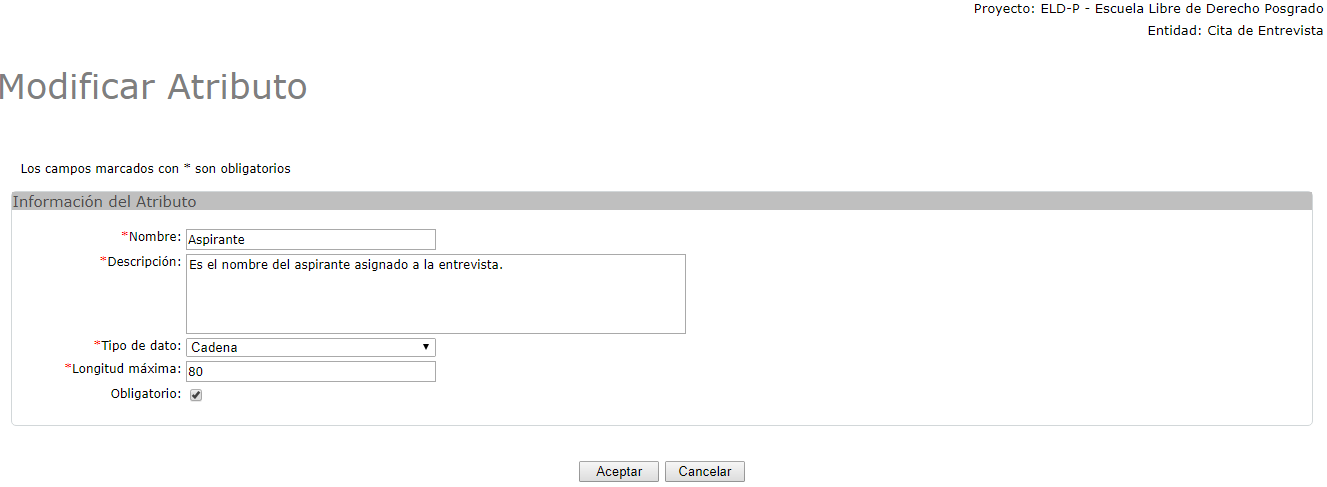
\includegraphics[scale=0.5]{roles/lider/entidades/atributos/pantallas/IU12-1-2modificarAtributo}
					\caption{Modificar Atributo}
					\label{fig:modificarAtributo}
				\end{center}
			\end{figure}
		
			\item Modifique los datos solicitados por la pantalla.
			
			\item Dependiendo del tipo de dato que elija aparecerán nuevos campos que son requeridos para el tipo de dato seleccionado. Las siguientes pantallas muestran los campos que requiere cada tipo de dato:
			
			\begin{figure}[H]
				\begin{center}
					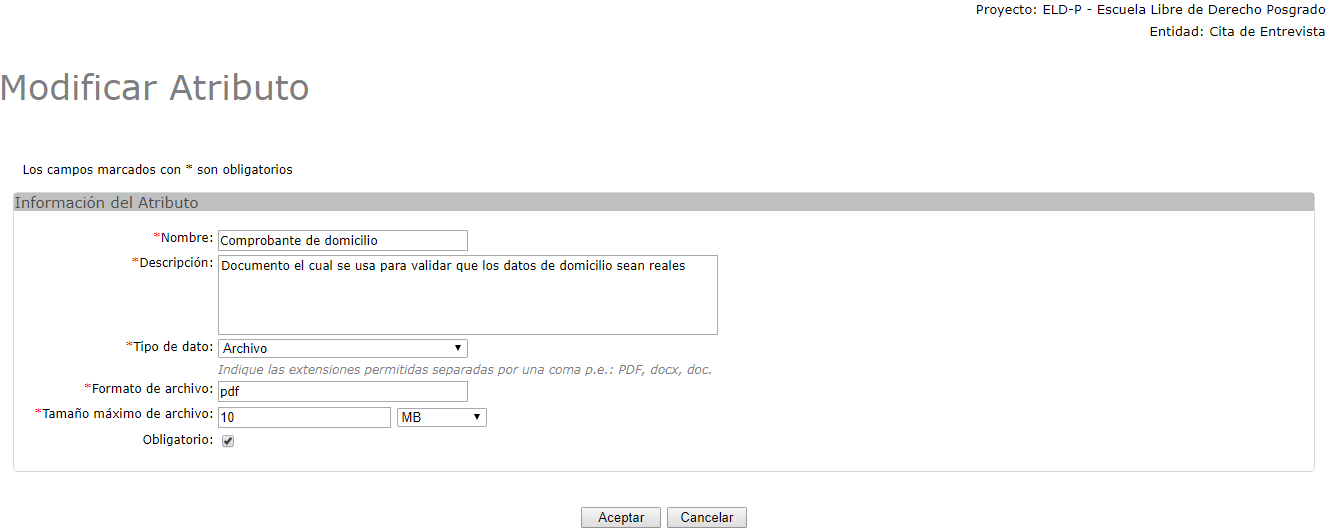
\includegraphics[scale=0.5]{roles/lider/entidades/atributos/pantallas/IU12-1-2AmodificarAtributo}
					\caption{Modificar Atributo: Archivo}
					\label{fig:modificarAtributoA}
				\end{center}
			\end{figure}
			
			\begin{figure}[H]
				\begin{center}
					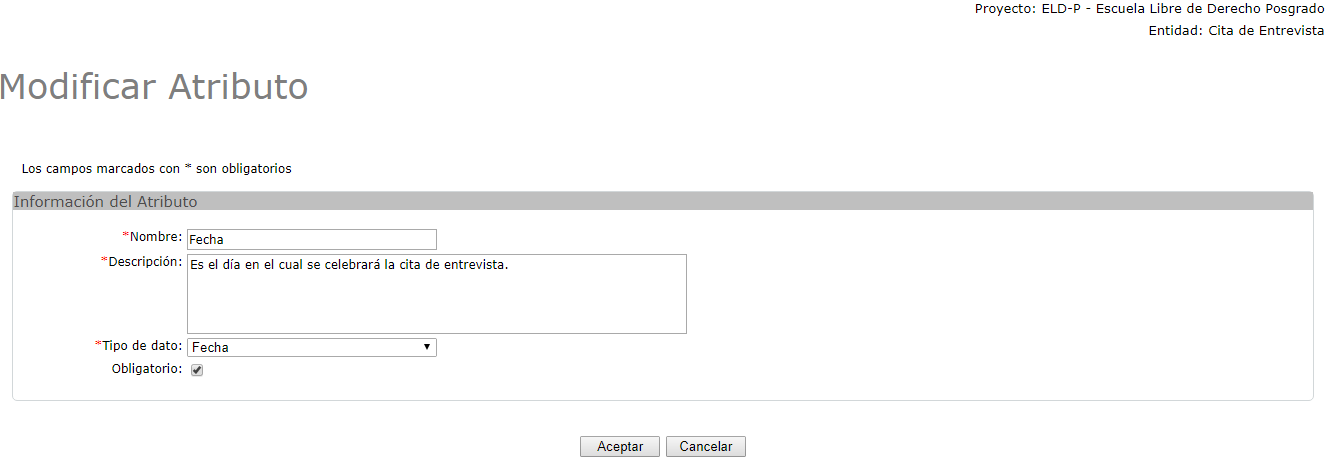
\includegraphics[scale=0.5]{roles/lider/entidades/atributos/pantallas/IU12-1-2BmodificarAtributo}
					\caption{Modificar Atributo: Fecha}
					\label{fig:modificarAtributoB}
				\end{center}
			\end{figure}
			
			\begin{figure}[H]
				\begin{center}
					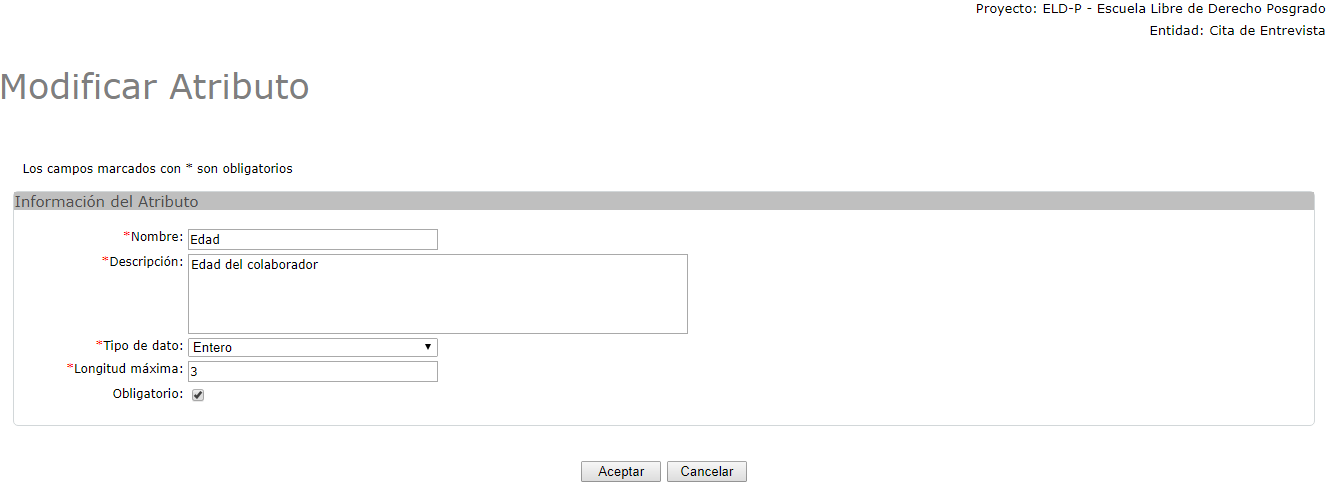
\includegraphics[scale=0.5]{roles/lider/entidades/atributos/pantallas/IU12-1-2CmodificarAtributo}
					\caption{Modificar Atributo: Entero}
					\label{fig:modificarAtributoC}
				\end{center}
			\end{figure}
			
			\begin{figure}[H]
				\begin{center}
					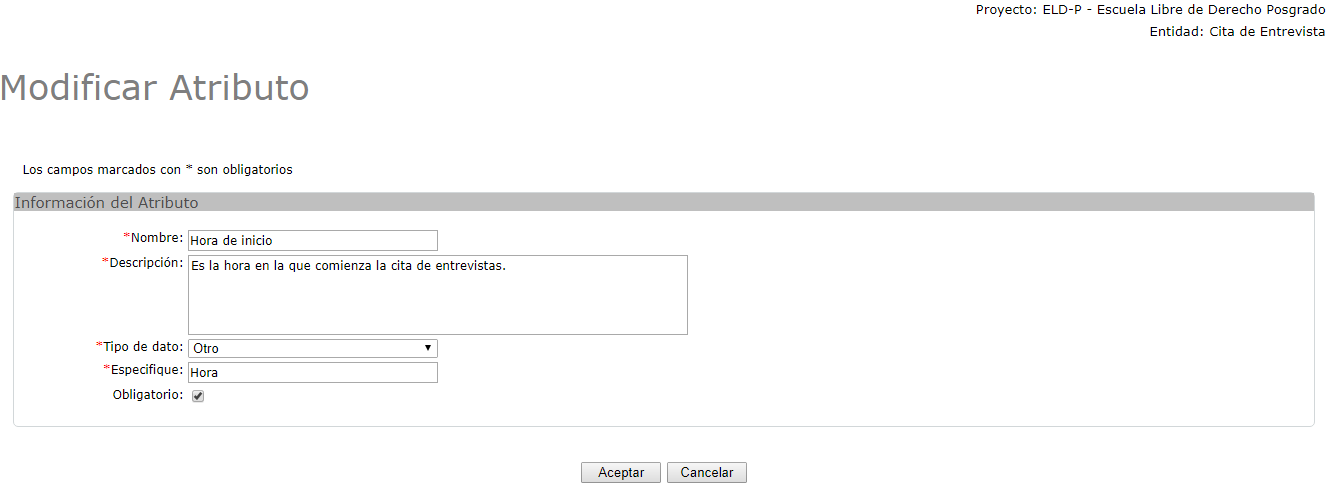
\includegraphics[scale=0.5]{roles/lider/entidades/atributos/pantallas/IU12-1-2DmodificarAtributo}
					\caption{Modificar Atributo: Otro}
					\label{fig:modificarAtributoD}
				\end{center}
			\end{figure}
						
			\item Oprima el botón \IUAceptar.
			
			\item Se mostrará el mensaje \ref{fig:atributoModificado} en la pantalla \ref{fig:GestionarAtributos} ''Gestionar Atributos''.
			
			\begin{figure}[htbp!]
				\begin{center}
					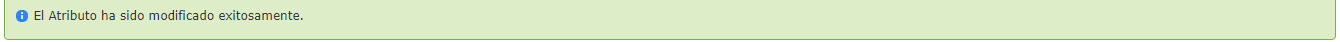
\includegraphics[scale=0.5]{roles/lider/entidades/atributos/pantallas/IU12-1-2MSG1}
					\caption{MSG: Atributo Actualizado}
					\label{fig:atributoModificado}
				\end{center}
			\end{figure}
			\end{enumerate}